\documentclass[presentation]{beamer}

\usepackage{tikz}
\usetikzlibrary{positioning,calc}
\usetikzlibrary{shapes.geometric}
\usetikzlibrary{backgrounds}% only to show the bounding box
\usetikzlibrary{shapes,arrows}
\usepackage{pgfplots}
\usepackage{pgfplotstable}
\usetikzlibrary{pgfplots.groupplots}
\pgfplotsset{compat=1.12}
\usepackage{appendixnumberbeamer}
\usepackage{amsmath}
\date{27th March 2017}
\usetheme{metropolis}
\usepackage{pifont}

\newcommand{\cmark}{\ding{51}}
\newcommand{\xmark}{\ding{55}}

\titlegraphic{\hfill\includegraphics[height=2em]{imperial-bw-gray}}
\metroset{progressbar=frametitle}

\renewcommand{\vec}[1]{\ensuremath{\boldsymbol{#1}}}
\newcommand{\ddt}[1]{\frac{\partial #1}{\partial t}}
\newcommand{\zhat}{\hat{\vec{z}}}
\newcommand{\W}{\ensuremath{\mathbb{W}}}

\DeclareMathOperator{\grad}{grad}
\let\div\relax
\DeclareMathOperator{\div}{div}
\DeclareMathOperator{\curl}{curl}
\newcommand{\vsubset}[1]{\rotatebox[origin=c]{90}{\ensuremath{\subset}}}
\newcommand{\inner}[2]{\ensuremath{\langle #1, #2 \rangle}}
\author{Lawrence Mitchell\inst{1}}
\institute{
\inst{1}Departments of Computing and Mathematics, Imperial College
London
}

\graphicspath{{./\jobname.figures/}}

\newcommand{\arxivlink}[2]{%
  \href{http://www.arxiv.org/abs/#1}%
  {{\small\texttt{arXiv:\,#1\,[#2]}}}%
}
\newcommand{\doilink}[1]{%
  \href{http://dx.doi.org/#1}%
  {{\small\texttt{doi:\,#1}{}}}%
}

\usepackage[url=false,
doi=true,
isbn=false,
style=authoryear,
firstinits=true,
uniquename=init,
backend=biber]{biblatex}


\setbeamertemplate{bibliography item}{}
\renewcommand{\bibfont}{\footnotesize}
\addbibresource{references.bib}

\setlength{\bibitemsep}{1ex}

\renewbibmacro{in:}{}
\DeclareFieldFormat[article]{volume}{\textbf{#1}}
\DeclareFieldFormat{doi}{%
  doi\addcolon%
  {\scriptsize\ifhyperref{\href{http://dx.doi.org/#1}{\nolinkurl{#1}}}
    {\nolinkurl{#1}}}}
\AtEveryBibitem{%
\clearfield{pages}%
\clearfield{issue}%
\clearfield{number}%
}

\usepackage{minted}
\usepackage{cancel}
\title{From here to there}
\subtitle{challenges for \cancel{peta} exa-scale transient simulation}

\begin{document}

\maketitle

\begin{frame}[standout]
  50GHz single-core CPUs
\end{frame}

\section{The status quo}

\begin{frame}
  \frametitle{What we have to work with}
  \begin{tabular}{lccccc}
    Chip & Cores & TF/s & GB/s & F/B & Power \\
    \hline
    NVidia P100 & 56 (3584) & 5.3 & 730 & 7.2 & 250 (21 GF/W) \\
    Xeon Phi 7290F & 72 & 3.5 & 450 & 7.8 & 260 (13 GF/W) \\
    Broadwell & 22 & 0.78 & 150 & 5.2 & 140 (5.6 GF/W)
  \end{tabular}

  \begin{block}{Exascale}
    \begin{itemize}
    \item<1-> 190K NVidia P100s, 1e9-way concurrency, 50MW
    \item<1-> 290K Intel Phis, 1e8-way concurrency, 75MW
    \item<1-> 1.3M Intel Broadwells, 3e7-way concurrency, 180MW
    \item<2-> 1 Boeing 747, 140MW
    \item<3-> 1 Sizewell B, 1200MW
    \item<4-> 1 UK, 35GW
    \end{itemize}
  \end{block}
  % NVIDIA P100 (Pascal) 56 SMTs 5.3TF/s 732GB/s (16GB) 7.2F/B 250W 21F/W

  % Intel Xeon Phi 7290F 72 cores 3.5TF/s ~450GB/s (16GB) 7.8F/B 260W 13F/W

  % Intel Broadwell E5-2699v4 22 cores 0.78TF/s 150GB/s (<1.5TB) 5.2F/B
  % 140W 5.6F/W
\end{frame}

\begin{frame}[standout]
 Run LINPACK
\end{frame}

\begin{frame}
  \frametitle{But seriously}
  \begin{itemize}
  \item High useful arithmetic intensity (flops are cheaper than bytes)
  \item Vectorise, vectorise, vectorise (only way to achieve flops)
  \item Avoid bulk synchronous computation (performance resilience)
  \item Reduce and/or amortise communication (hide latency)
  \end{itemize}
\end{frame}

\begin{frame}
  \frametitle{Current codes}

  \begin{itemize}
  \item[\xmark] Typically low order, memory-bound
  \item[\xmark] Vectorisation left to compiler (?)
  \item[\xmark] Iterative schemes with blocking reductions
  \item[\xmark] Simple communication patterns (not optimal?)
  \end{itemize}
\end{frame}


\section{Is my code any good?}

\begin{frame}
  \frametitle{Algorithmically}

  \begin{block}{Notation}
  $N$ -- total number of degrees of freedom;

  $P$ -- total number of processes;

  $T(N, P)$ -- time to solution.
  \end{block}

  \begin{block}{Good}
    $\mathcal{O}(N)$ computational complexity;

    $\mathcal{O}(\log P)$ communication complexity.

    Actually care about minimal $T$, so $\mathcal{O}(N\log N)$ can be good.
  \end{block}
\end{frame}

\begin{frame}
  \frametitle{Scalability}

  \begin{block}{Weak scaling}
    Constant local work $N/P$.

    Scalable code has $T(N, P) = T(2N, 2P)$.
  \end{block}

  \begin{block}{Strong scaling}
    Decreasing local work $N/P$.

    Scalable code has $T(N, P) = 2T(N, 2P)$.
  \end{block}

  \begin{onlyenv}<2>
    Time-resolved transient simulations do not weak scale. Sad!
  \end{onlyenv}
\end{frame}


\begin{frame}
  \frametitle{What is good?}

  Summarising \textcite{Fischer:2015}\footnote{\citefield{Fischer:2015}{doi}}.
  
  \begin{block}{}

    $T_a(N, P) = T_a(N, 1)/P$ -- parallelisable work;

    $T_c(N, P)$ -- communication;

    $c$ -- serial overhead.

    \begin{equation*}
      T(N, P) = \left\{
        \begin{split}
          &T_a(N, P) + T_c(N, P) + c &\text{ synchronous comms}\\
          &\max(T_a(N, P), T_c(N, P)) + c\,\,&\text{ asynchronous comms}
        \end{split}\right.
    \end{equation*}

    $\eta = T(N, 1)/(PT(N,P)$ -- strong scaling efficiency.
  \end{block}
\end{frame}

\begin{frame}
  \frametitle{When to stop?}

  Bigger problems need more timesteps.
  
  To maintain time to solution as $N\rightarrow \infty$, need strong
  scaling.

  \begin{block}{Cost efficiency}
    Ignore $c$ (reasonable for CPUs for a good code).

    Often $P_{\text{opt}}$ when $T_a(N, P_\text{opt}) = T_c(N,
    P_\text{opt})$, $\eta = 0.5$.
  \end{block}

  \begin{block}{Folk lemma}
    Krylov methods strong scale to $N/P \approx 30000$.
  \end{block}
\end{frame}

\begin{frame}
  \frametitle{Measuring $P_{\text{opt}}$}
  
  \begin{itemize}
  \item Measure $T(N, 1)$, $T(N, P)$, for a range of $P$.

  \item Find $P_\text{opt}$ such that
    $P_\text{opt}T(N, P_\text{opt}) = 2T(N,1)$.

  \item How do I know if that is objectively optimal?

  \item<2>{Build a model.}
  \end{itemize}
\end{frame}

\begin{frame}
  \frametitle{Building blocks}
  \begin{block}{Computation}
    Measure $S$, e.g., flops with $P=1$, $N$ large.

    ``atomic'' unit of computation takes time $t_a = S^{-1}$.
  \end{block}

  \begin{block}{Communication}
    Linear model, latency + bandwidth.

    Time (s) to send $m$ doubles
    \begin{equation*}
      t_c(m) = \alpha^* + \beta^* m
    \end{equation*}
    non-dimensionalise, $\alpha = \alpha^*/t_a$, $\beta =
    \beta^*/t_a$.
    \begin{equation*}
      t_c(m) = (\alpha + \beta m)t_a
    \end{equation*}
  \end{block}
\end{frame}

\begin{frame}
  \frametitle{Is this a good model?}
  \begin{center}
    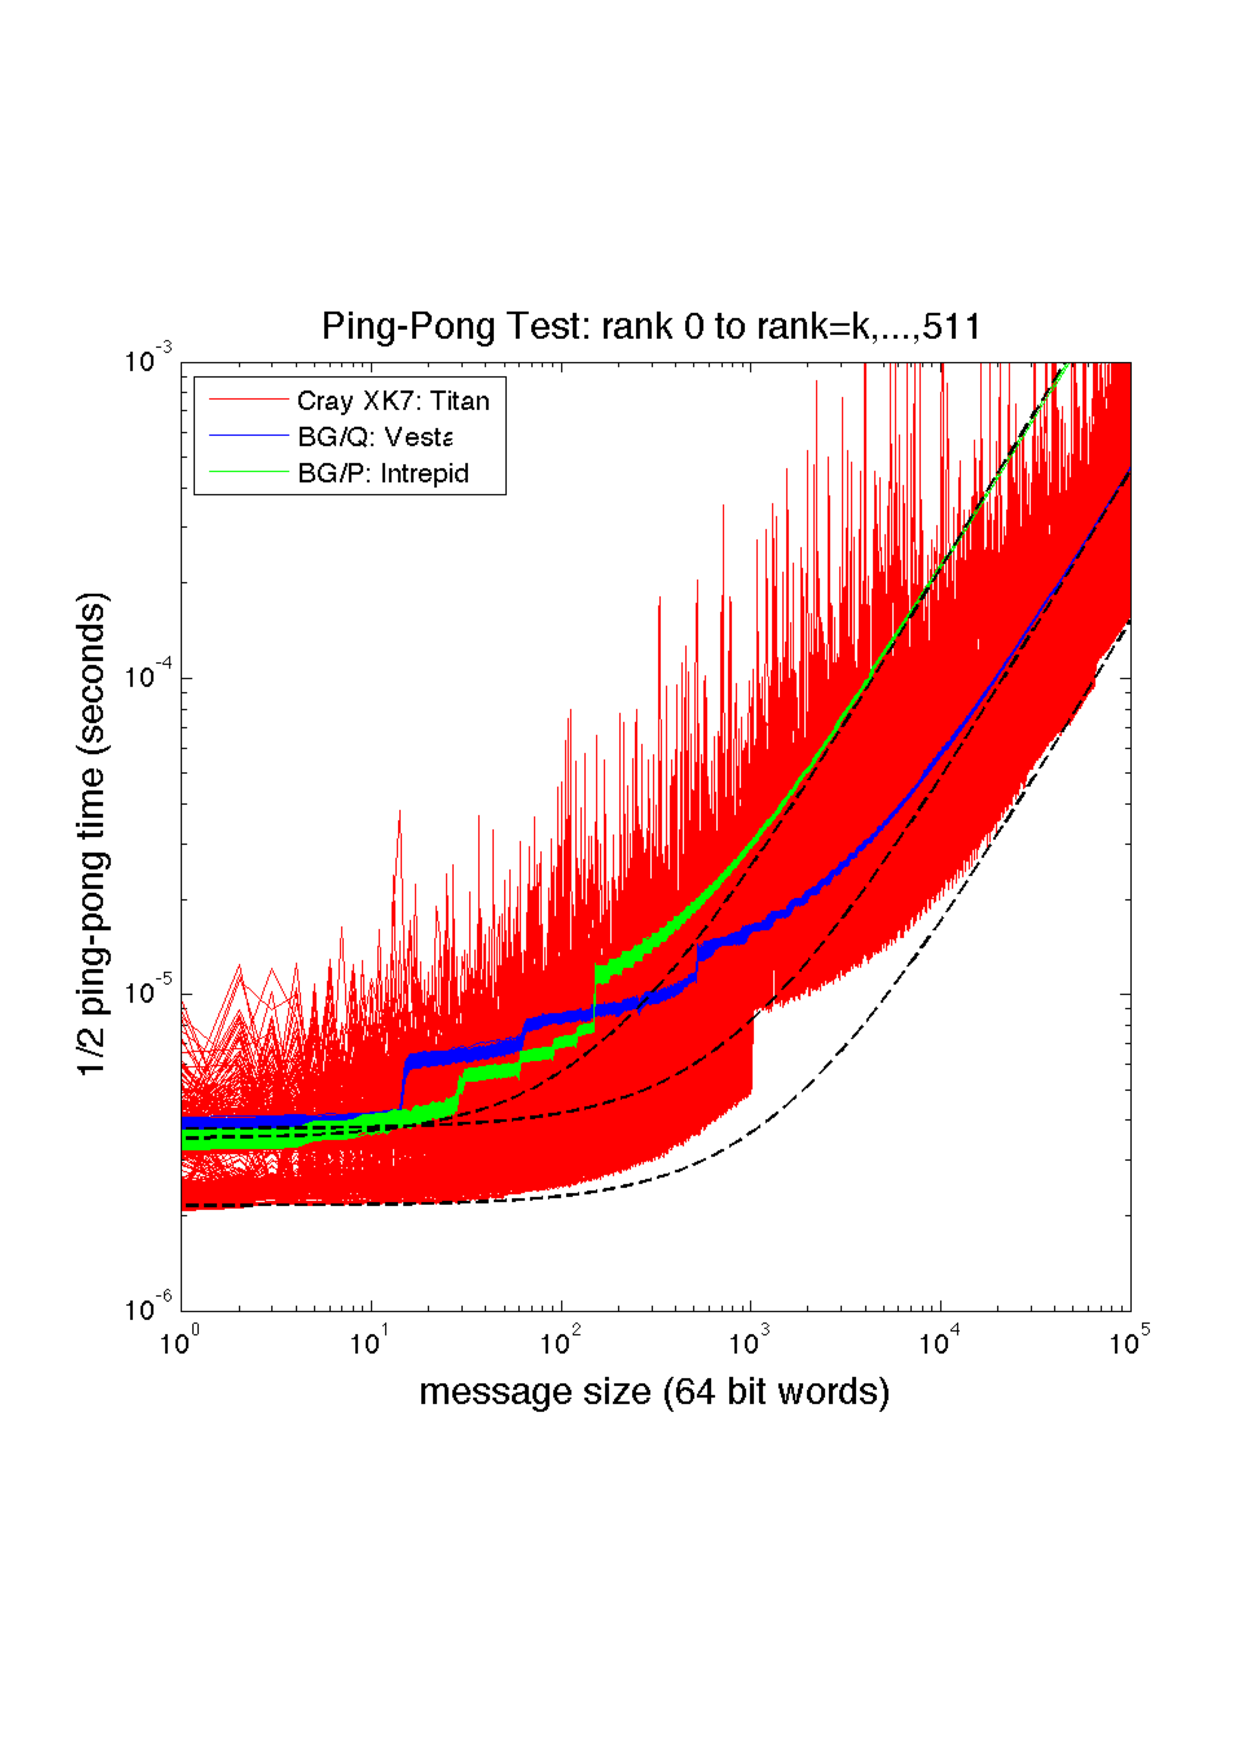
\includegraphics[height=0.8\textheight]{ping-pong}
  \end{center}
  From \textcite{Fischer:2015}.

\end{frame}

\begin{frame}
  \frametitle{Jacobi iteration}
  \begin{equation*}
    u_i^{k+1} = a_{ii}^{-1}\left(f_i + \sum_{j \ne i} a_{ij}u_j^{k}\right)
  \end{equation*}
  counting operations with $N/P$ entries per process, for a 7 point stencil.
  \begin{equation*}
    T_a = 14(N/P)t_a.
  \end{equation*}
  With a block decomposition, each face exchange moves $(N/P)^{2/3}$
  values, so
  \begin{equation*}
    T_c = 6 \left(\alpha + \beta (N/P)^{2/3}\right)t_a.
  \end{equation*}

  With $\alpha = 3750, \beta = 2.86$ (BG/Q), $T_a = T_c$ when $N/P
  \approx 1700$.  \emph{Independent} of $P$.

  If $\beta = 0$, $N/P \approx 1600$.
\end{frame}


\begin{frame}
  \frametitle{Conjugate gradients}
  For a 7 point stencil, we do 27 operations per dof
  \begin{equation*}
    T_a = 27(N/P) t_a
  \end{equation*}
  With a block decomposition, we again need 6 face exchanges, plus
  two reductions
  \begin{equation*}
    T_c = 6 \left(\alpha + \beta (N/P)^{2/3}\right)t_a + 2 \cdot 2 \log_2 P \alpha t_a.
  \end{equation*}

  Now the scaling limit is $P$-dependent.

  \begin{itemize}
    \item $P=10^6$: $N/P \approx 12000$;
    \item $P=10^9$: $N/P \approx 17000$.
  \end{itemize}

  Reasonably well aligned with the folk lemma.
\end{frame}

\begin{frame}
  \frametitle{But wait}
  \begin{center}
    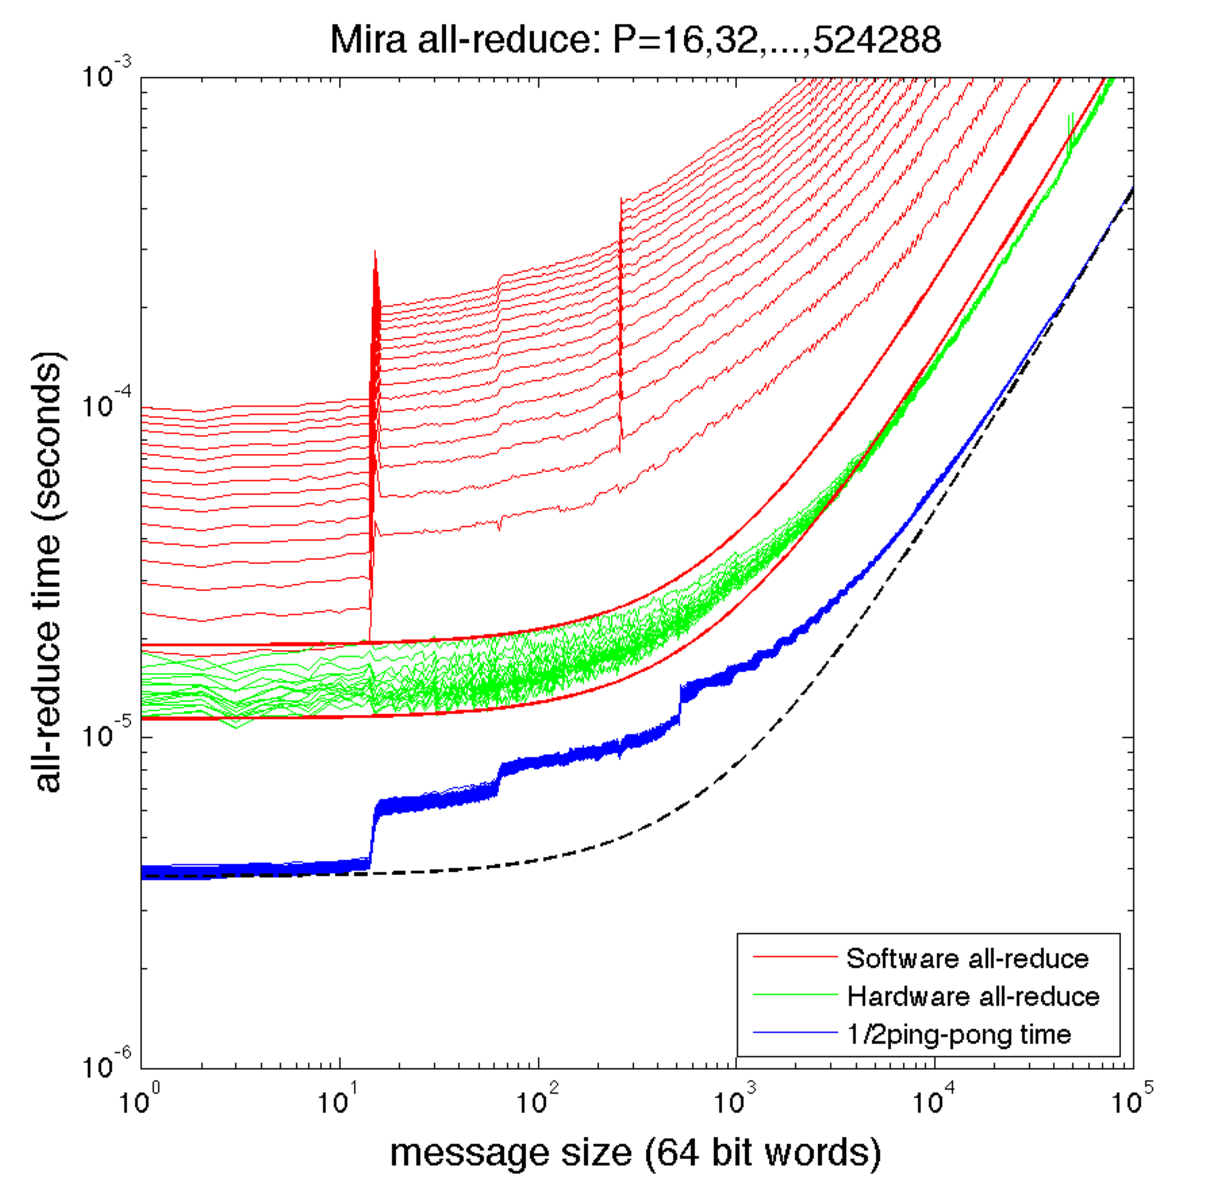
\includegraphics[height=0.8\textheight]{allreduce}
  \end{center}
  From \textcite{Fischer:2015}.
\end{frame}

\begin{frame}
  \frametitle{Round again}
  \begin{equation*}
    T_c = 6 \left(\alpha + \beta (N/P)^{2/3}\right)t_a +
    \cancel{2\cdot 2 \log_2 P \alpha t_a} + 2 \cdot 5 \alpha t_a.
  \end{equation*}

  Now we have $P$-\emph{independent} scaling behaviour, $N/P \approx 2100$.

  Using only a single reduction, we can get to $N/P \approx
  1500$.

  \alert{8x} more strong scaling on $P=10^9$.

  A similar analysis can be done for multilevel algorithms,
  e.g.~Poisson $N/P \approx 7500$, or $N\approx 10^{12}$ on an exascale
  system.
\end{frame}

\begin{frame}
  \frametitle{Latency hurts}

  \begin{itemize}
  \item When strong-scaling mesh codes, you don't care about network
    bandwidth.
  \item Decreasing $\alpha$ is important, pester your vendor!
  \item Faster cores (relative to network) means worse strong scaling.
  \item Faster code means worse strong scaling.
  \end{itemize}
\end{frame}

\begin{frame}
  \frametitle{Something to aim at}

  \begin{onlyenv}<1>
    3-D incompressible Navier-Stokes for reactor cooling, NEK5000.

    \begin{center}
      \includegraphics[height=0.6\textheight]{nek-strong-scale}

      Data reproduced from \textcite{Fischer:2015}.
    \end{center}
  \end{onlyenv}

  \begin{onlyenv}<2>
    3-D non-hydrostatic baroclinic instability 3km resolution, Gordon Bell prize
    2016.
    \begin{center}
      \includegraphics[height=0.6\textheight]{sunway-strong-scale}

      Data reproduced from \textcite{Yang:2016}.
    \end{center}
  \end{onlyenv}
\end{frame}

\begin{frame}
  \frametitle{Some thoughts on climate codes}

  \begin{block}{Conjecture}
    Most (all?) full climate models are nowhere near optimal use of current
    hardware.

    Extrapolating current SYPD to larger problems is perhaps not
    useful, unless we think the current models are good.
  \end{block}

  \begin{itemize}
  \item More work means scaling should improve.
  \item Will column-wise data decomposition start to hurt?
  \item Lobby for power spend on interconnect, not cores?
  \item Don't forget to focus on minimising time-to-solution first.
  \end{itemize}
\end{frame}

\section{What might we do?}

\begin{frame}
  \frametitle{Improving SYPD}

  Better serial performance.  Is it the case that current codes make
  efficient use of hardware?

  High order?  Only useful if we can use fewer dofs.  Are models in
  the asymptotic region where we expect exponential accuracy gains
  from high order discretisations?

  Better strong scaling.  Necessary to counteract timestep
  restrictions with increasing resolution.
\end{frame}

\begin{frame}
  \frametitle{Better serial performance}

  Ground up rewrites of models?

  Local optimisations are difficult to do, because typically we need
  to make global changes in data layout.  If data model is implicit,
  this is bad.
  
  Look for opportunities to reduce algorithmic complexities

  \textcite{Yang:2016} is an example of what you can do for a single
  component.
  
\end{frame}

\begin{frame}
  \frametitle{Addressing latency}

  Remove communication (possible with some multilevel methods,
  c.f. $\tau$-FAS)

  Amortise latency.  We're not network bandwidth limited, so ``tile''
  in time (obvious how this works for explicit schemes).  Some work
  from Qiqi Wang, also the ``diamond tiling'' literature (Hager/Keyes,
  ...).

  Basically, do one 10m byte exchange every 10 steps, rather than 10 m
  byte exchanges.  Cost: $\alpha + 10 \beta m$, rather than $10(\alpha
  + \beta m)$.
\end{frame}

\begin{frame}
  \frametitle{Putting physics back in}
  Will help strong scaling (more local work)

  At some point, if we want more small timescales to be resolved, we
  need time parallel (at high resolution).

  Is higher resolution the best thing to do?  Better spin up/data
  assimilation.  More ensembles?  Better statistics?
\end{frame}

\appendix
\begin{frame}[t,allowframebreaks]
  \frametitle{References}
  
  \printbibliography[heading=none]
\end{frame}
\end{document}
